\documentclass[12pt,reqno]{article}
\usepackage[english]{babel}
\usepackage{url}
\usepackage[utf8]{inputenc}
\usepackage{amsmath}
\usepackage{graphicx}
\graphicspath{{figs/}}
\usepackage{parskip}
\usepackage{fancyhdr}
\usepackage{vmargin}
\usepackage{appendix}
\usepackage{float}
\usepackage{booktabs}
\usepackage{caption}
\usepackage{subfig}
\usepackage{bm}
\usepackage{listings}
\usepackage{array}
\usepackage{hyperref}
\usepackage[normalem]{ulem}

% \hypersetup{
%     colorlinks=true,
%     linkcolor=blue,  
%     urlcolor=blue,
% }

\newcommand{\stkout}[1]{\ifmmode\text{\sout{\ensuremath{#1}}}\else\sout{#1}\fi}
\newcolumntype{P}[1]{>{\centering\arraybackslash}p{#1}}
\setmarginsrb{3 cm}{2.5 cm}{3 cm}{2.5 cm}{1 cm}{1.5 cm}{1 cm}{1.5 cm}

\newcounter{eqn}
\renewcommand*{\theeqn}{\alph{eqn})}
\newcommand{\numtwo}{\refstepcounter{eqn}\text{\theeqn}\;}

\makeatletter
\newcommand{\putindeepbox}[2][0.7\baselineskip]{{%
    \setbox0=\hbox{#2}%
    \setbox0=\vbox{\noindent\hsize=\wd0\unhbox0}
    \@tempdima=\dp0
    \advance\@tempdima by \ht0
    \advance\@tempdima by -#1\relax
    \dp0=\@tempdima
    \ht0=#1\relax
    \box0
}}
\makeatother

\lstset{language=Python,%
    %basicstyle=\color{red},
    breaklines=true,%
    morekeywords={matlab2tikz},
    keywordstyle=\color{blue},%
    morekeywords=[2]{1}, keywordstyle=[2]{\color{black}},
    identifierstyle=\color{black},%
    stringstyle=\color{mylilas},
    commentstyle=\color{mygreen},%
    showstringspaces=false,%without this there will be a symbol in the places where there is a space
    numbers=left,%
    numberstyle={\tiny \color{black}},% size of the numbers
    numbersep=9pt, % this defines how far the numbers are from the text
    emph=[1]{for,end,break},emphstyle=[1]\color{red}, %some words to emphasise
    %emph=[2]{word1,word2}, emphstyle=[2]{style},    
}

\title{ECE 459 - Assignment 4} % Title

\author{}
\date{\today} % Date

\makeatletter
\let\thetitle\@title
\let\theauthor\@author
\let\thedate\@date
\makeatother

\pagestyle{fancy}
\fancyhf{}
\rhead{\theauthor}
\lhead{\thetitle}
\cfoot{\thepage}

\begin{document}

% custom commands 
\newcommand{\units}[1]{$\hspace{0.25em}\mathrm{[#1]}$}

%%%%%%%%%%%%%%%%%%%%%%%%%%%%%%%%%%%%%%%%%%%%%%%%%%%%%%%%%%%%%%%%%%%%%%%%%%%%%%%%%%%%%%%%%

\begin{titlepage}
	\centering
    \vspace*{-1 cm}
    
\includegraphics[scale = 0.5]{images/UW.jpg}\\	% University Logo
	\rule{\linewidth}{0.2 mm} \\[0.4 cm]
	{ \huge \bfseries \thetitle}\\
	\rule{\linewidth}{0.2 mm} \\[1.5 cm]
	
	\begin{minipage}[t]{0.4\textwidth}
		\begin{flushleft} \large
			\emph{Author:}\\
            David Chau \\
			\end{flushleft}
			\end{minipage}~
			\begin{minipage}[t]{0.4\textwidth}
			\begin{flushright} \large
			\emph{Student Number:} \\
            20623345\\
		\end{flushright}
	\end{minipage}\\[2 cm]
	Date: 
	{\large March 30, 2020}\\[2 cm]
	\vfill
\end{titlepage}

%%%%%%%%%%%%%%%%%%%%%%%%%%%%%%%%%%%%%%%%%%%%%%%%%%%%%%%%%%%%%%%%%%%%%%%%%%%%%%%%%%%%%%%%%

\section*{Profiling}
The task for this assignment was to optimize the performance of a given simulation of a Hackathon. Analysis was done using flamegraphs to identify bottlenecks in the program and corresponding corrections to the code were implemented. After a correction was made, a new flamegraph was generated to be used as the next starting point of investigation. In the end, the following areas were investigated and corrected: 
\begin{enumerate}
    \item \texttt{Container} class in \texttt{Container.h}
    \item \texttt{xorChecksum()} function in \texttt{utils.cpp}
    \item \texttt{readFileLine()} used by \texttt{PackageDownloader::run()}
    \item \texttt{getNextIdea()} used by \texttt{IdeaGenerator::run()}
\end{enumerate}

The first problem to fix was the \texttt{Container} class. This was primarily indicated by the \texttt{crossProduct} function which showed that its usage of \texttt{Container<StrPair>::push} accounted for a significant amount of CPU time. To optimize this, the internal storage being used by the \texttt{Container} class was replaced by \texttt{std::deque}, which provided more efficient access to stored data. The results of this, relative to \texttt{hackathon\_slow}, can be seen in Table \ref{tab:first-fix}.

\begin{table}[H]
    \centering
    \caption{Results from optimizing the \texttt{Container} class}
    \label{tab:first-fix}
    \begin{tabular}{|P{3.0cm}|P{3.0cm}|P{3.0cm}|P{3.0cm}|}
    \hline
    \textbf{}& \textbf{\# Samples} & \textbf{CPU Time} & \textbf{ Runtime (s)}\\ \hline 
    Before & 3027 & 33.79\% & 1.837 \\ \hline
    After & 28 & 0.50\% & 1.007 \\ \hline
    \end{tabular}
\end{table}

The second problem was identified as the inefficiency of the algorithm used by \\ \texttt{xorChecksum}. Initially, it was performing 32 iterations, which processed 8 bits at a time. A solution was attempted in which only 4 iterations were required, processing 64 bits at a time. The speedup was deemed insufficient, with the bottleneck being the usage of \texttt{std::stringstream}. Finally, a solution which avoids using \texttt{std::stringstream} was implemented. The results from this, relative to the last fix, can be seen in Table \ref{tab:second-fix}.

\begin{table}[H]
    \centering
    \caption{Results from optimizing \texttt{xorChecksum()}}
    \label{tab:second-fix}
    \begin{tabular}{|P{3.0cm}|P{3.0cm}|P{3.0cm}|P{3.0cm}|}
    \hline
    \textbf{}& \textbf{\# Samples} & \textbf{CPU Time} & \textbf{ Runtime (s)}\\ \hline 
    Before & 1465 & 26.08\% & 1.007 \\ \hline
    After & 34 & 1.18\% & 0.3994 \\ \hline
    \end{tabular}
\end{table} 

The next problem identified was the usage of \texttt{readFileLine()} in \\ \texttt{PackageDownloader::run()}. Essentially, every time a package name needed to be read from file, the file had to be re-opened and a sequential search for the specified line needed to be performed. This was changed by reading in the entire file once per thread and storing it in a \texttt{Container}. From here, package names were accessed through the \texttt{Container} using index manipulation. The results of this, relative to the last fix, can be seen in Table \ref{tab:third-fix}.

\begin{table}[H]
    \centering
    \caption{Results from optimizing \texttt{PackageDownloaer::run()}}
    \label{tab:third-fix}
    \begin{tabular}{|P{3.0cm}|P{3.0cm}|P{3.0cm}|P{3.0cm}|}
    \hline
    \textbf{}& \textbf{\# Samples} & \textbf{CPU Time} & \textbf{ Runtime (s)}\\ \hline 
    Before & 1647 & 56.79\% & 0.3994 \\ \hline
    After & 67 & 15.58\% & 0.2427 \\ \hline
    \end{tabular}
\end{table} 

The last problem identified was caused by \texttt{getNextIdea()} in \texttt{IdeaGenerator::run()}. In essence, each time an idea needed to be created, all the products and customers were read in and a cross product between them was performed. To correct this, each thread was made to only read in the products and customers once, with a following cross product also only being performed once. The results of this, relative to the last fix, can be seen in Table \ref{tab:fourth-fix}.

\begin{table}[H]
    \centering
    \caption{Results from optimizing \texttt{IdeaGenerator::run()}}
    \label{tab:fourth-fix}
    \begin{tabular}{|P{3.0cm}|P{3.0cm}|P{3.0cm}|P{3.0cm}|}
    \hline
    \textbf{}& \textbf{\# Samples} & \textbf{CPU Time} & \textbf{ Runtime (s)}\\ \hline 
    Before & 75 & 17.44\% & 0.2427 \\ \hline
    After & 14 & 3.00\% & 0.0570 \\ \hline
    \end{tabular}
\end{table} 

The aggregated results of testing using \texttt{hyperfine} with the default program arguments can be seen below in Table \ref{tab:hyperfine-results}. After all the optimizations were applied, the runtime of the program went from 1.837s to 0.057s, which is a 32x increase. As such, it can be concluded that the minimum required speed up was achieved.

\begin{table}[H]
    \centering
    \caption{Benchmark results for \texttt{hackathon} executions on \texttt{ecetesla0}}
    \label{tab:hyperfine-results}
    \begin{tabular}{|P{3cm}|P{2.5cm}|P{2.5cm}|P{2.5cm}|P{2.5cm}|}
    \hline
    \textbf{Test Case}& \textbf{Mean (s)} & \textbf{$\sigma$ (s)} & \textbf{Min (s)} & \textbf{Max (s)}\\ \hline 
    \texttt{hackathon\_slow} & 1.837 & 0.0360 & 1.792 & 1.892 \\ \hline
    \texttt{Fix \#1} & 1.007 & 0.032 & 0.968 & 1.060 \\ \hline
    \texttt{Fix \#2} & 0.3994 & 0.0703 & 0.3217 & 0.5459 \\ \hline
    \texttt{Fix \#3} & 0.2427 & 0.0765 & 0.1435 & 0.4382 \\ \hline
    \texttt{Fix \#4} & 0.057 & 0.0088 & 0.0384 & 0.0794 \\ \hline
    \end{tabular}
\end{table} 

Correspondingly, the final flamegraph can be seen in Figure \ref{fig:final-fg}. For the purpose of analysis, only call stacks above \texttt{runHackathon} were considered. In \texttt{hackathon\_slow}, the \texttt{runHackathon} function accounted for 7265 samples and  81.10\% of CPU time, whereas the final version of \texttt{hackathon\_fast} only accounted for 241 samples and 51.72\% of CPU time. This is validating of the fact that performance improvements were made between the two versions. With respect to further improvements, the final flamegraph indicates that the next areas to investigate are related to things such as file I/O and locking mechanisms.

\begin{figure}[H]
    \centering
    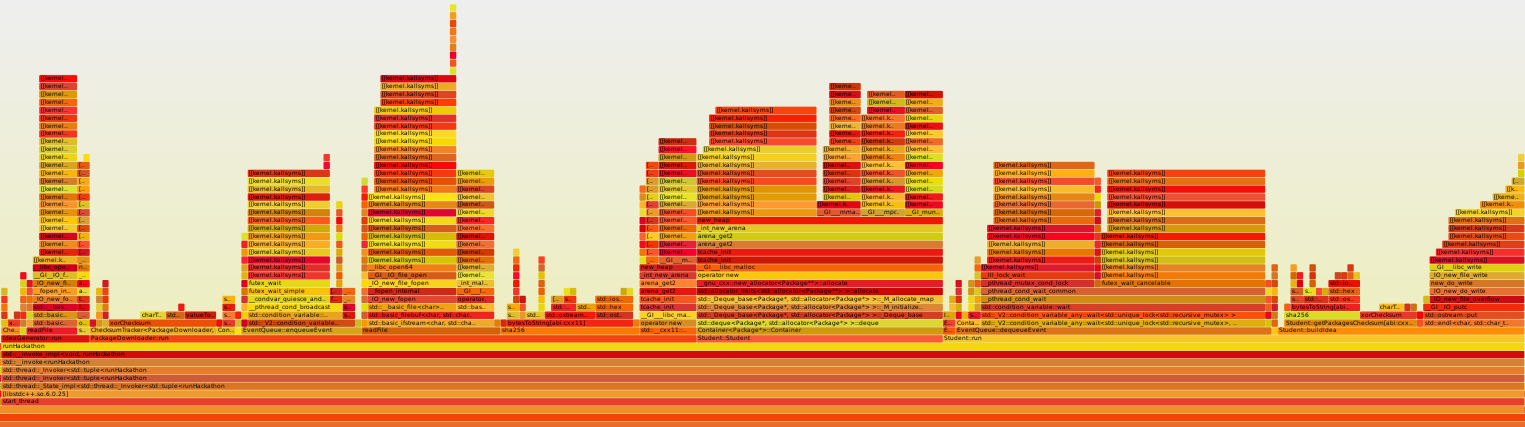
\includegraphics[width=1\textwidth]{images/final_fg.png}
    \caption{Relevant portion of final flamegraph showing \texttt{runHackathon}}
    \label{fig:final-fg}
\end{figure}


\clearpage
\pagebreak

\end{document}
